\section{设计结果}

\subsection{设计交付物}

\begin{verbatim}
|- score.xlsx              Excel：功能/性能测试得分
|- design.pdf              PDF：设计文档
|- .gitlab-ci.yml          CI/CD 配置
|-- src/
|    |-- mycpu/            我们的 CPU 完整源码
|    |    |-- xilinx_ip/   我们的 CPU 没有使用 IP 核 
|    |-- vivado_cannot/    无
|    |-- perf_clock.json   性能测试 CPU 主频
|-- bit/                   各项测试生成的 bit 文件
|-- show/                  决赛展示内容
\end{verbatim}

\subsection{CPU 功能与性能结果}

\begin{table}[H]
\centering
\caption{CPU 功能与性能测试结果}
\label{tab:perf}
\small
\begin{tabularx}{\textwidth}{>{\raggedright\arraybackslash}p{4.0cm}>{\raggedright\arraybackslash}p{4.0cm}X}
\toprule
项目 & 结果 & 说明 \\
\midrule
功能分 & \textbf{100.000000} & 58/58 点；最差 seed 通过，3/3 seed 通过 \\
IPC 比值 & \textbf{1.934633120} & IPC ratio \\
系统计数器比值 & \textbf{4.438258572} & system count ratio \\
最高实现频率 & \textbf{75.001875\,MHz} & \texttt{cpu\_clk} WNS $+0.052$\,ns \\
\bottomrule
\end{tabularx}
\end{table}

\subsection{linux启动}

\begin{figure}[H]
  \centering
  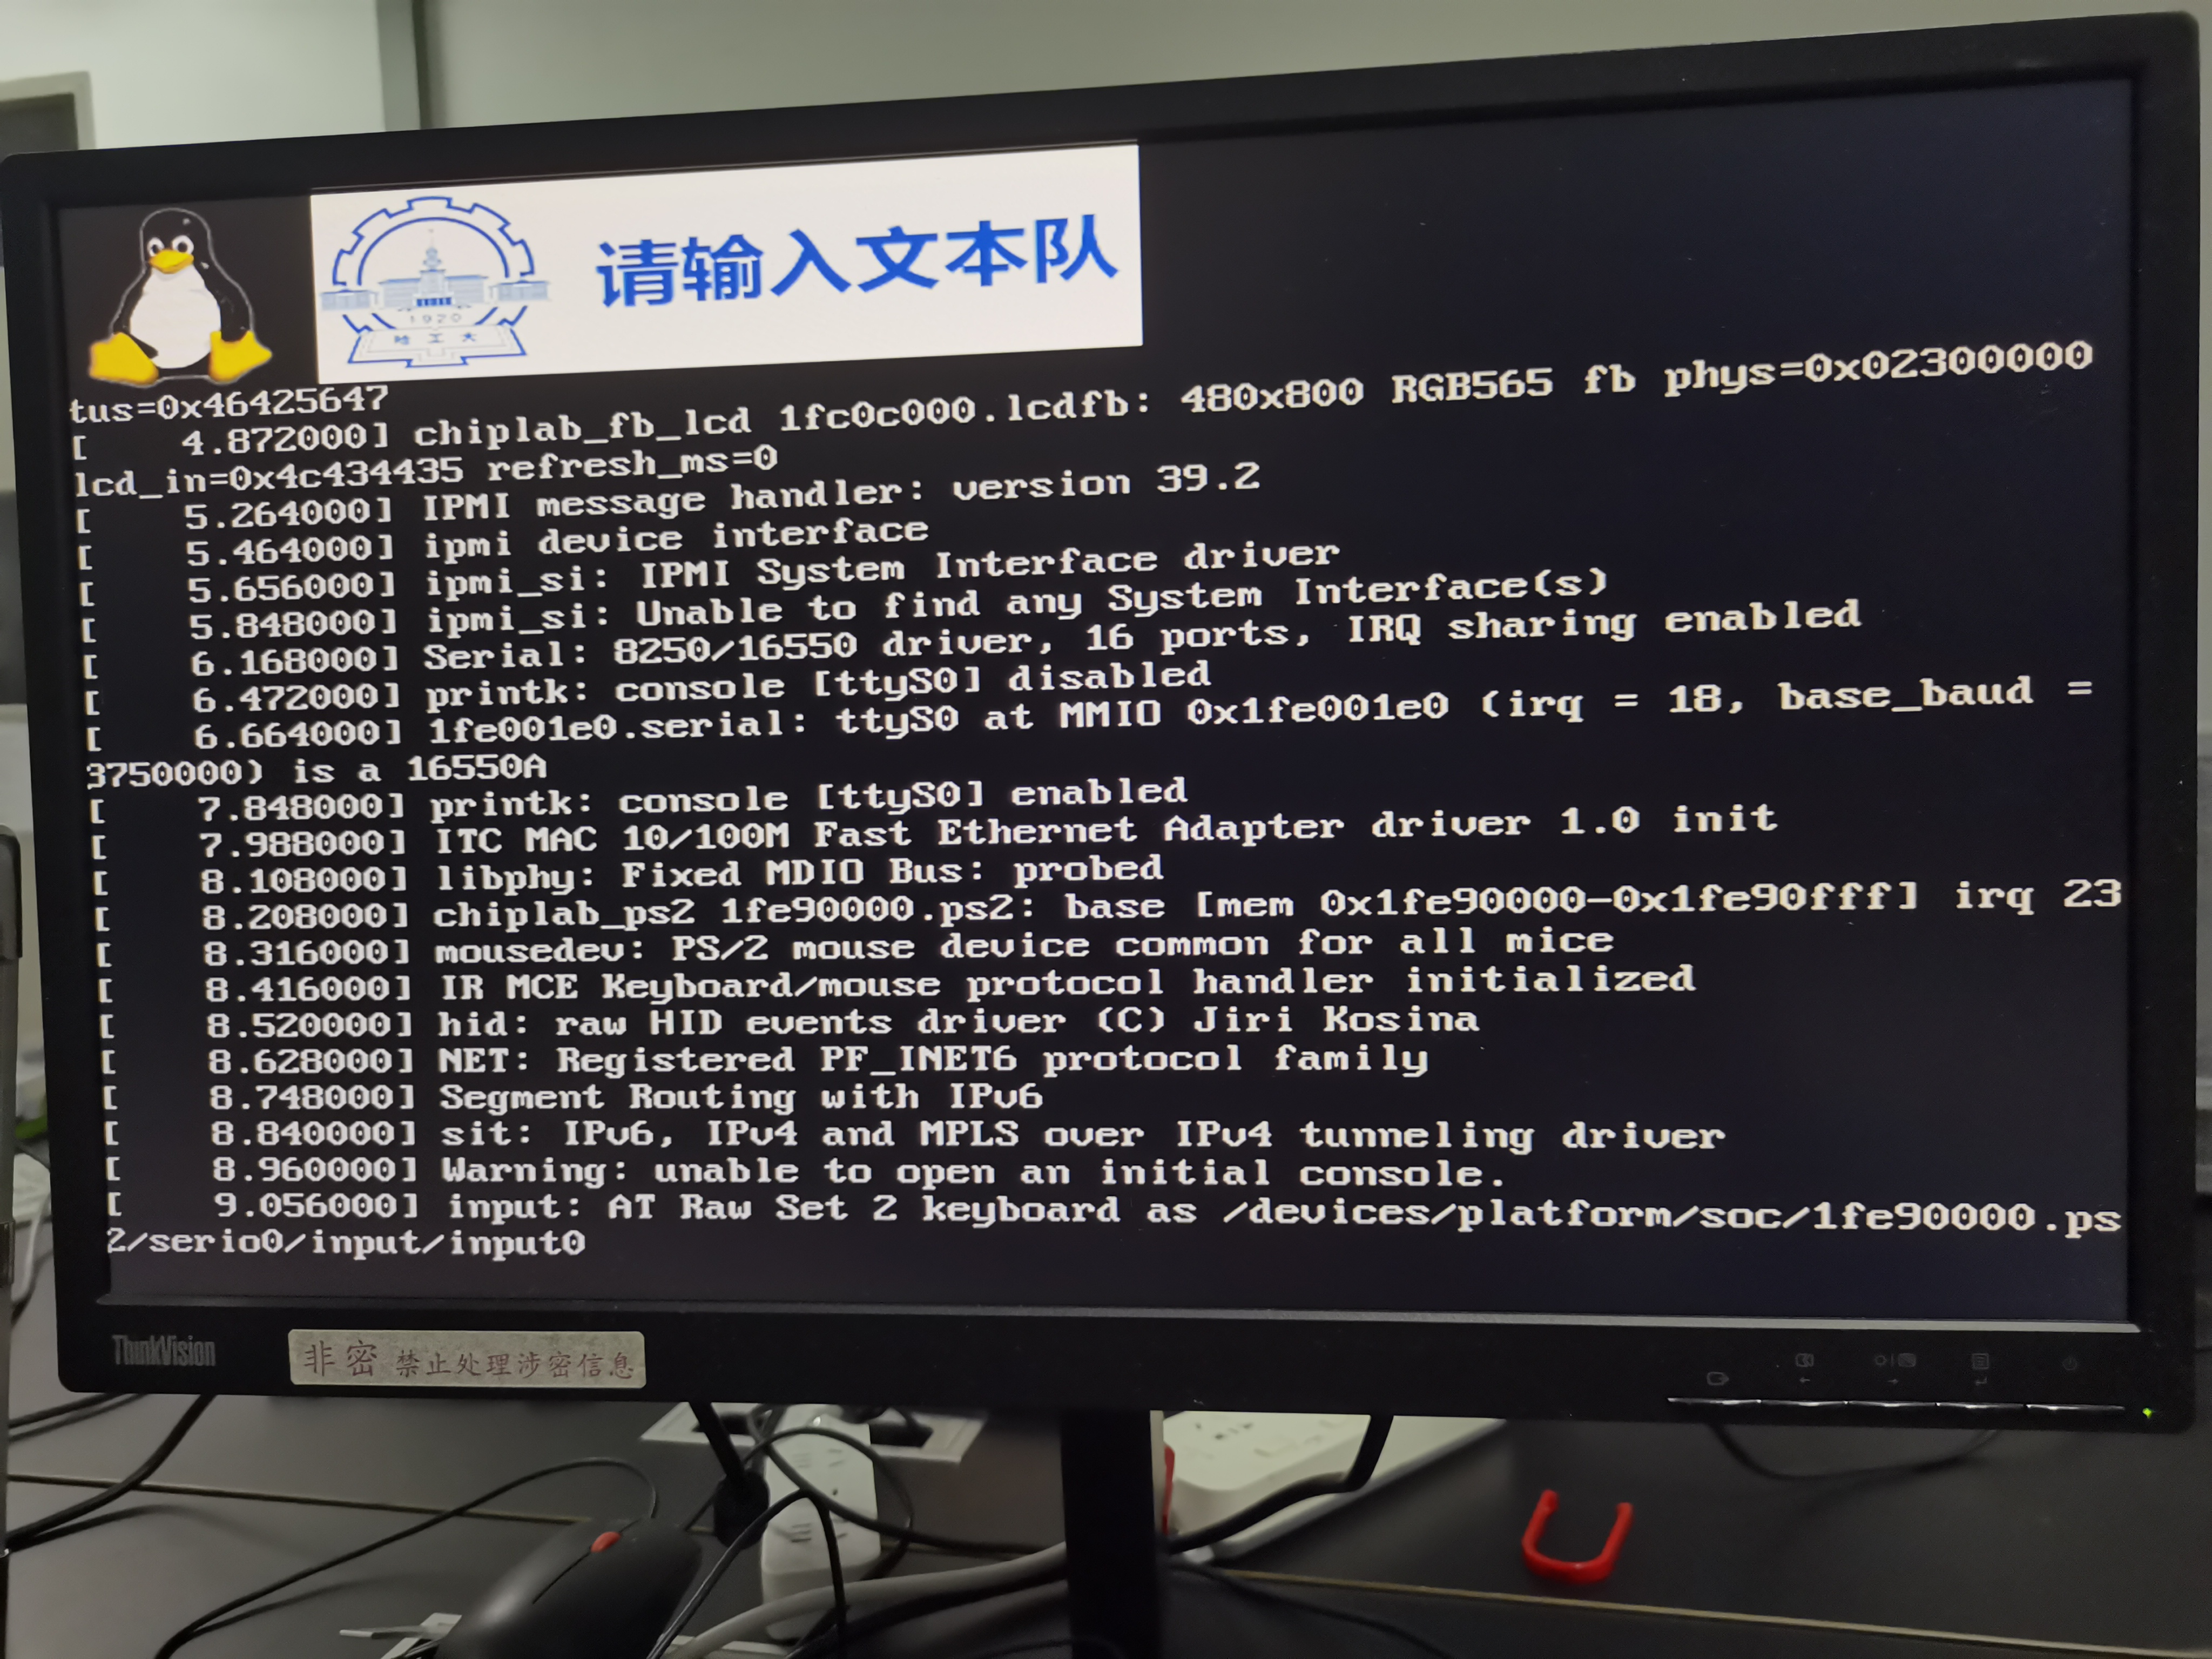
\includegraphics[width=0.95\textwidth]{figure/启动linux.jpg}
  \caption{linux启动}
  \label{fig:linux启动}
\end{figure}

